\documentclass[]{article}
\usepackage{graphicx}
\usepackage{indentfirst}
\usepackage{amsmath}
\usepackage{clrscode3e}
\setlength{\parindent}{0pt}


\title{HW07 for ECE 9343}
\author{Tongda XU, N18100977}

\begin{document}

\maketitle

\section{Question 1: CLRS Exercise 24.1-1}

From vertex z : See Figure ~\ref{fig:2411-1}\\
From vertex s : See Figure ~\ref{fig:2411-2}

\begin{figure}
	\centering
	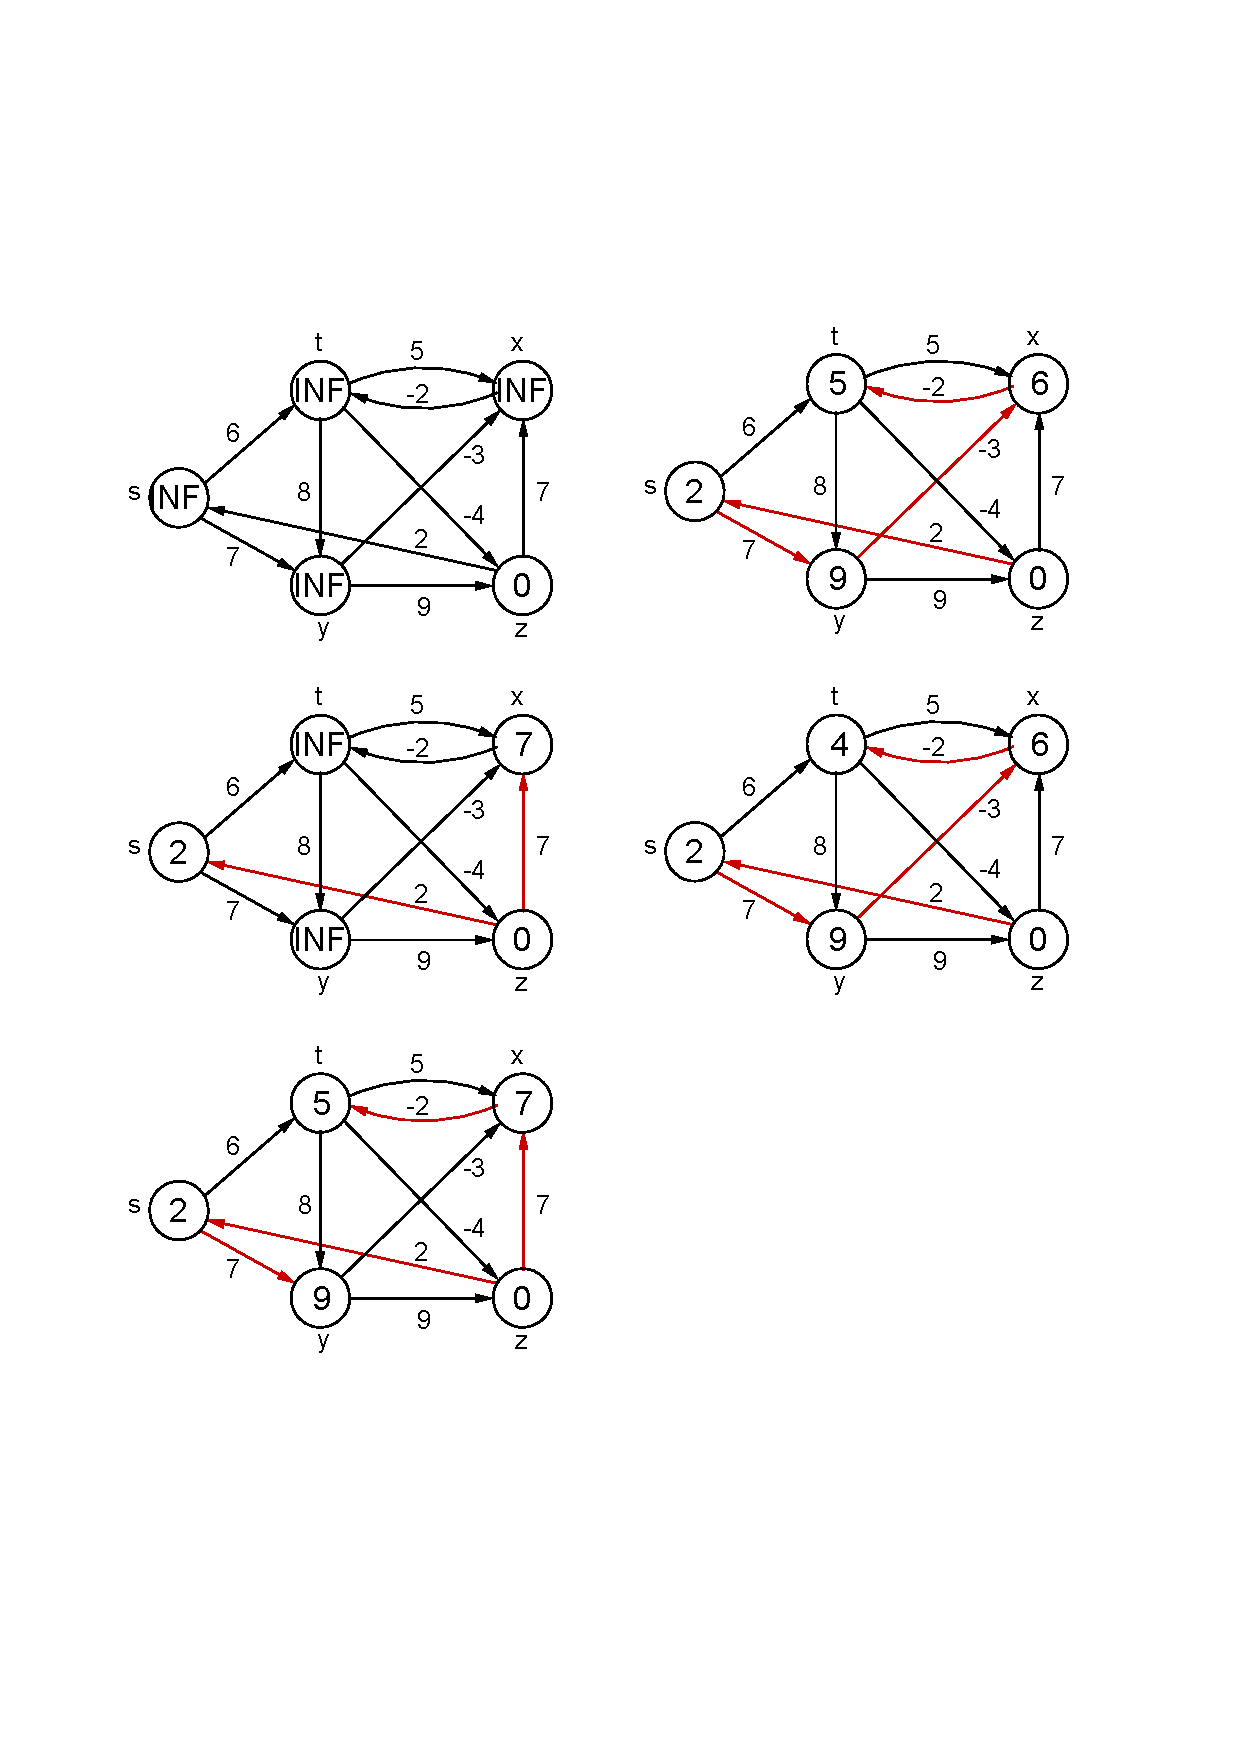
\includegraphics[width=\linewidth]{2411-1}
	\caption{Exercise 24.1-1, part1}
	\label{fig:2411-1}
\end{figure}

\begin{figure}
	\centering
	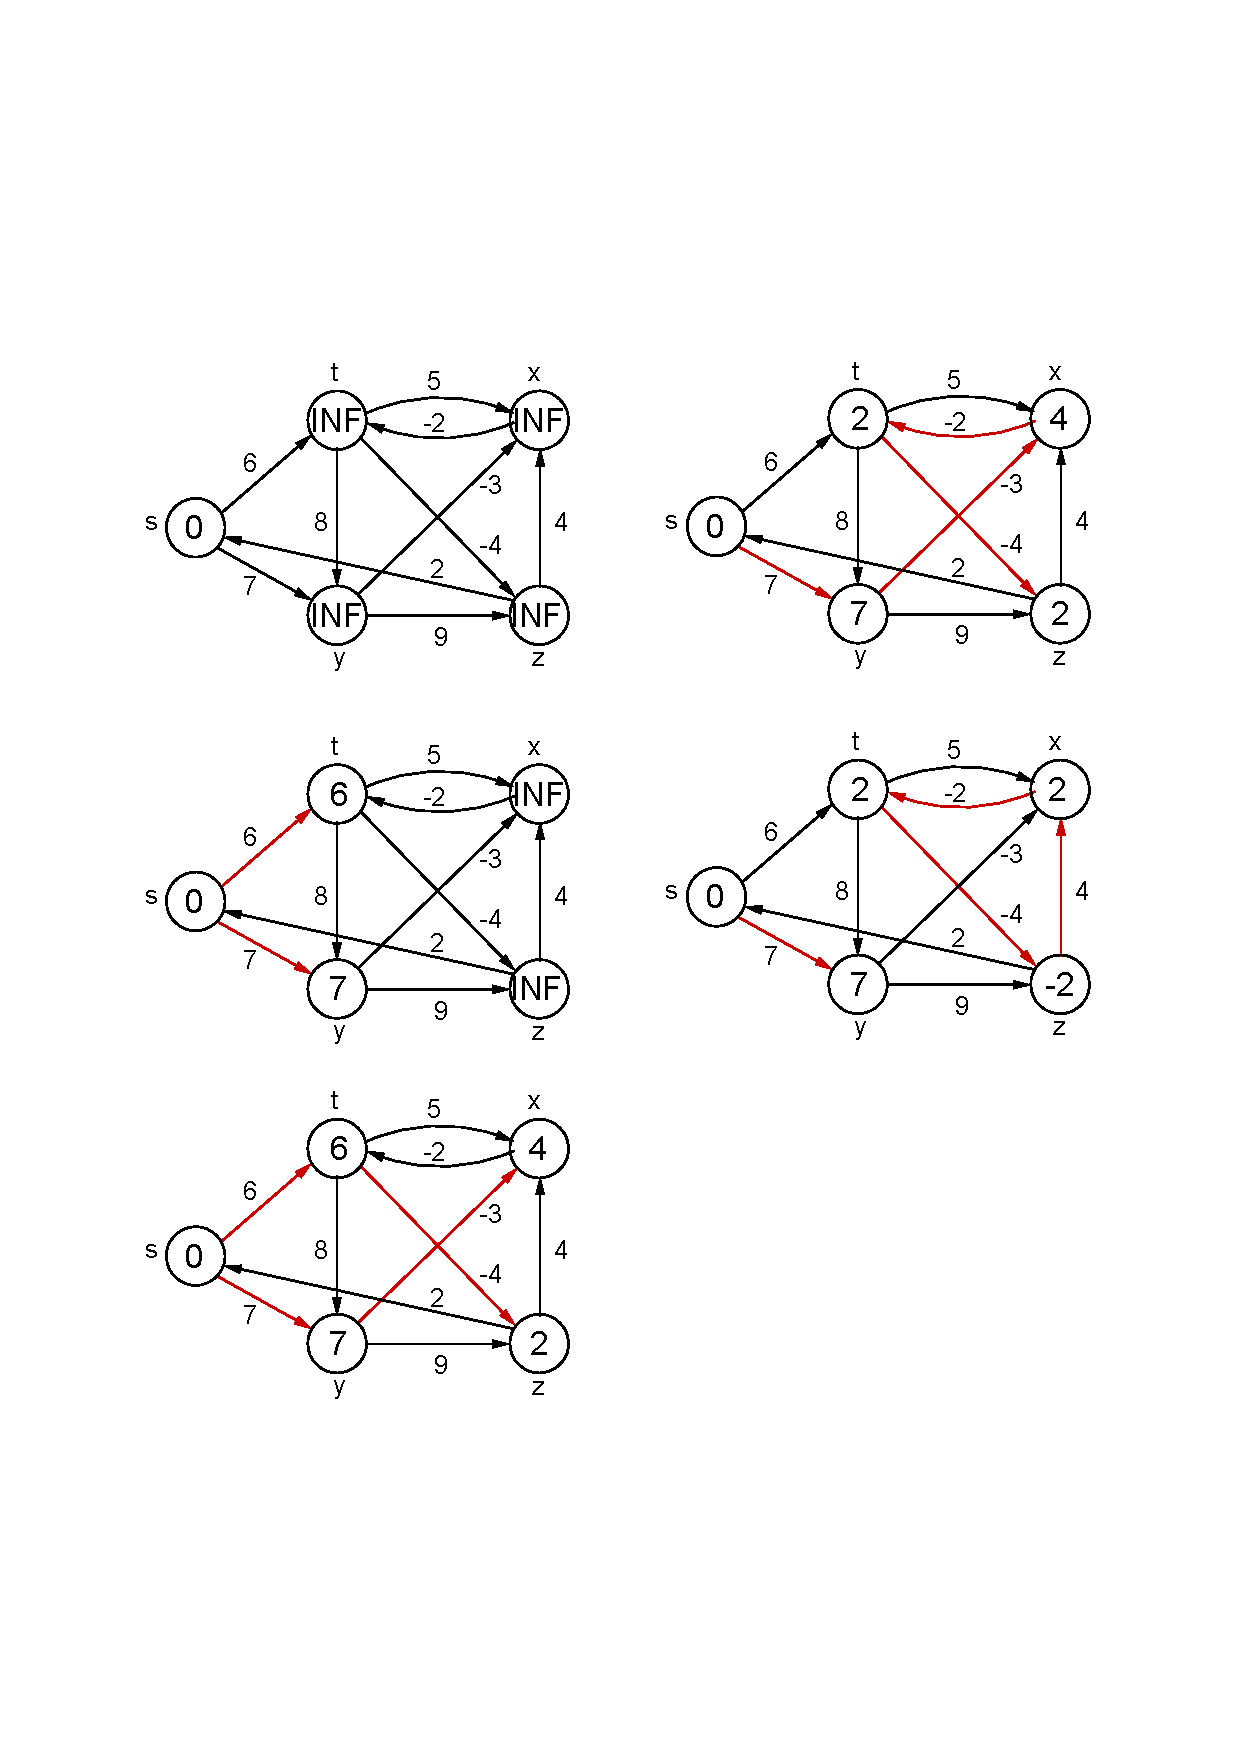
\includegraphics[width=\linewidth]{2411-2}
	\caption{Exercise 24.1-1, part2}
	\label{fig:2411-2}
\end{figure}


\section{Question 2: CLRS Exercise 24.2-1}

See Figure ~\ref{fig:2421}

\begin{figure}
	\centering
	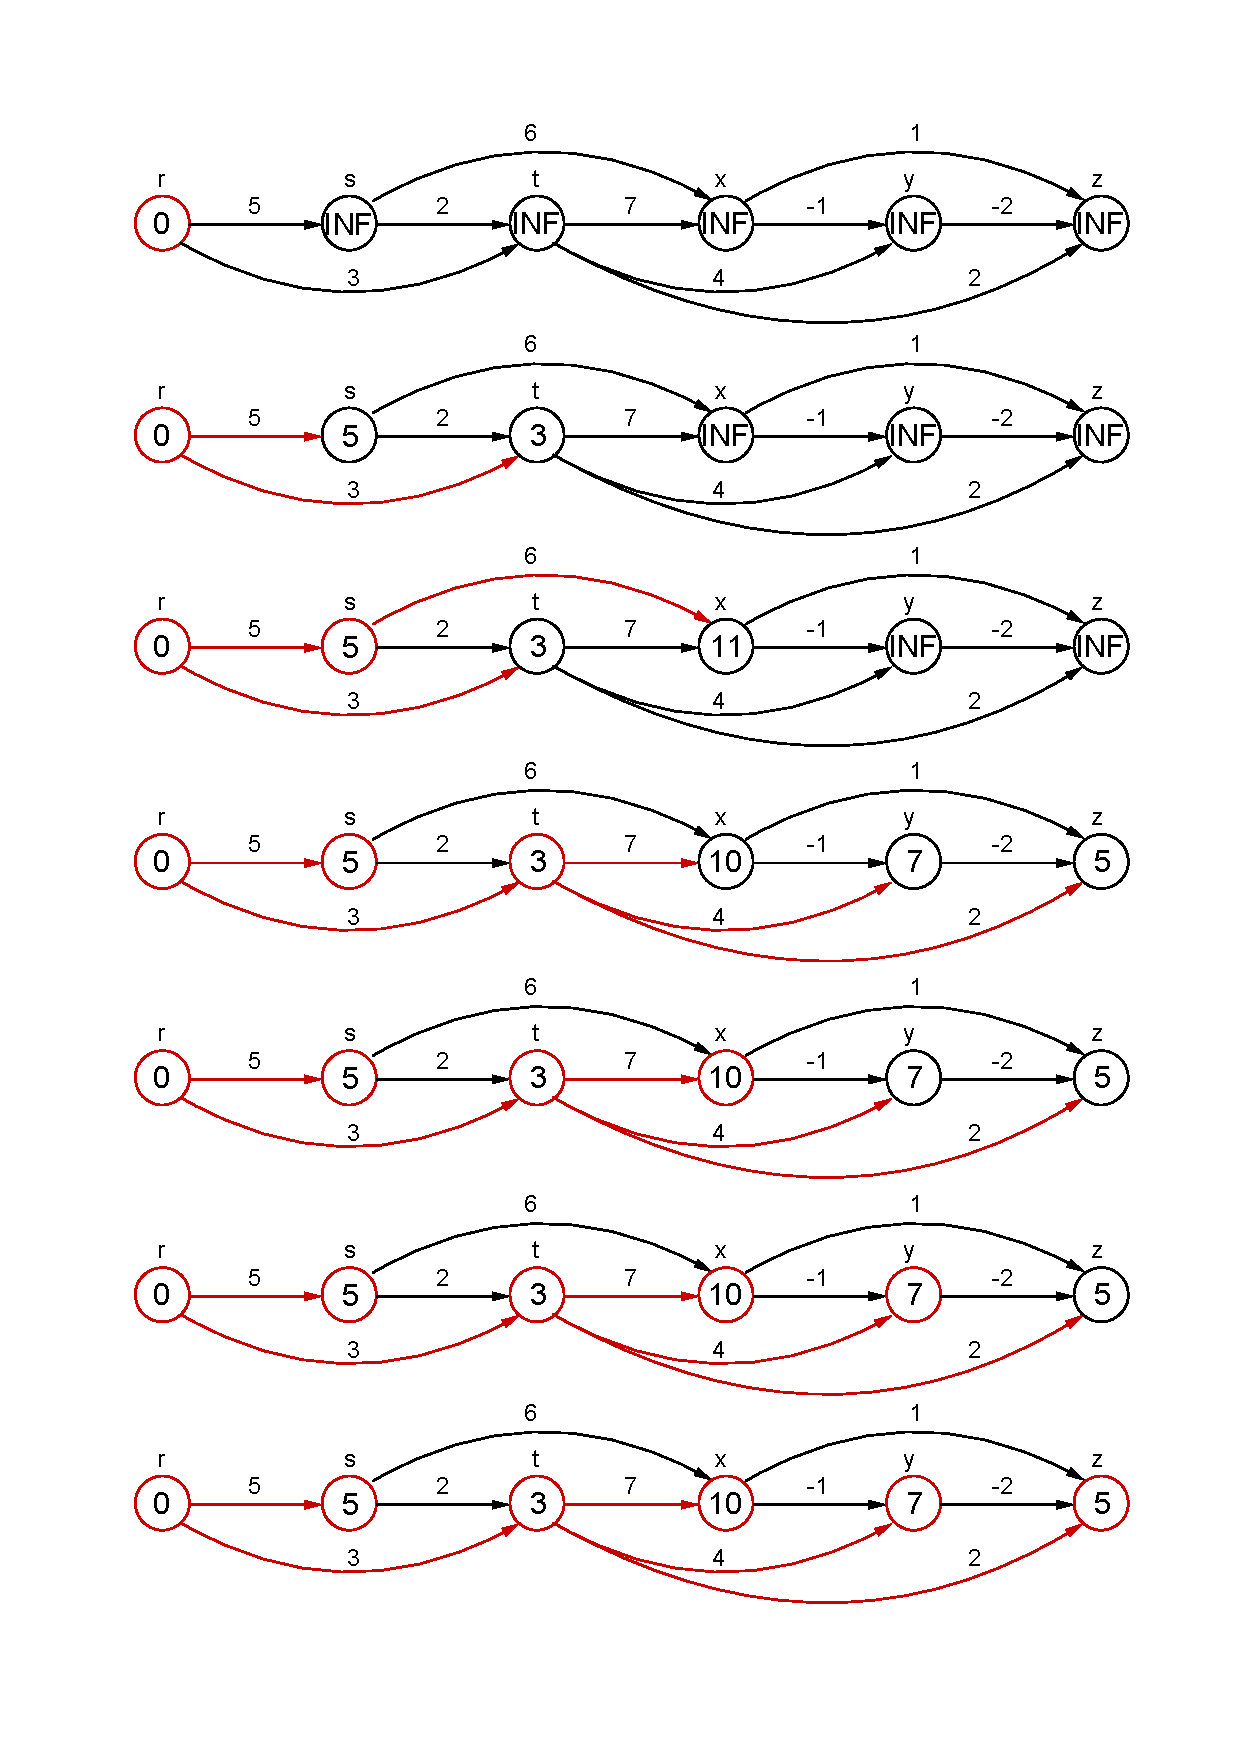
\includegraphics[width=\linewidth]{2421}
	\caption{Exercise 24.2-1}
	\label{fig:2421}
\end{figure}

\section{Question 3: CLRS Exercise 24.3-1}

See Figure ~\ref{fig:2431}

\begin{figure}
	\centering
	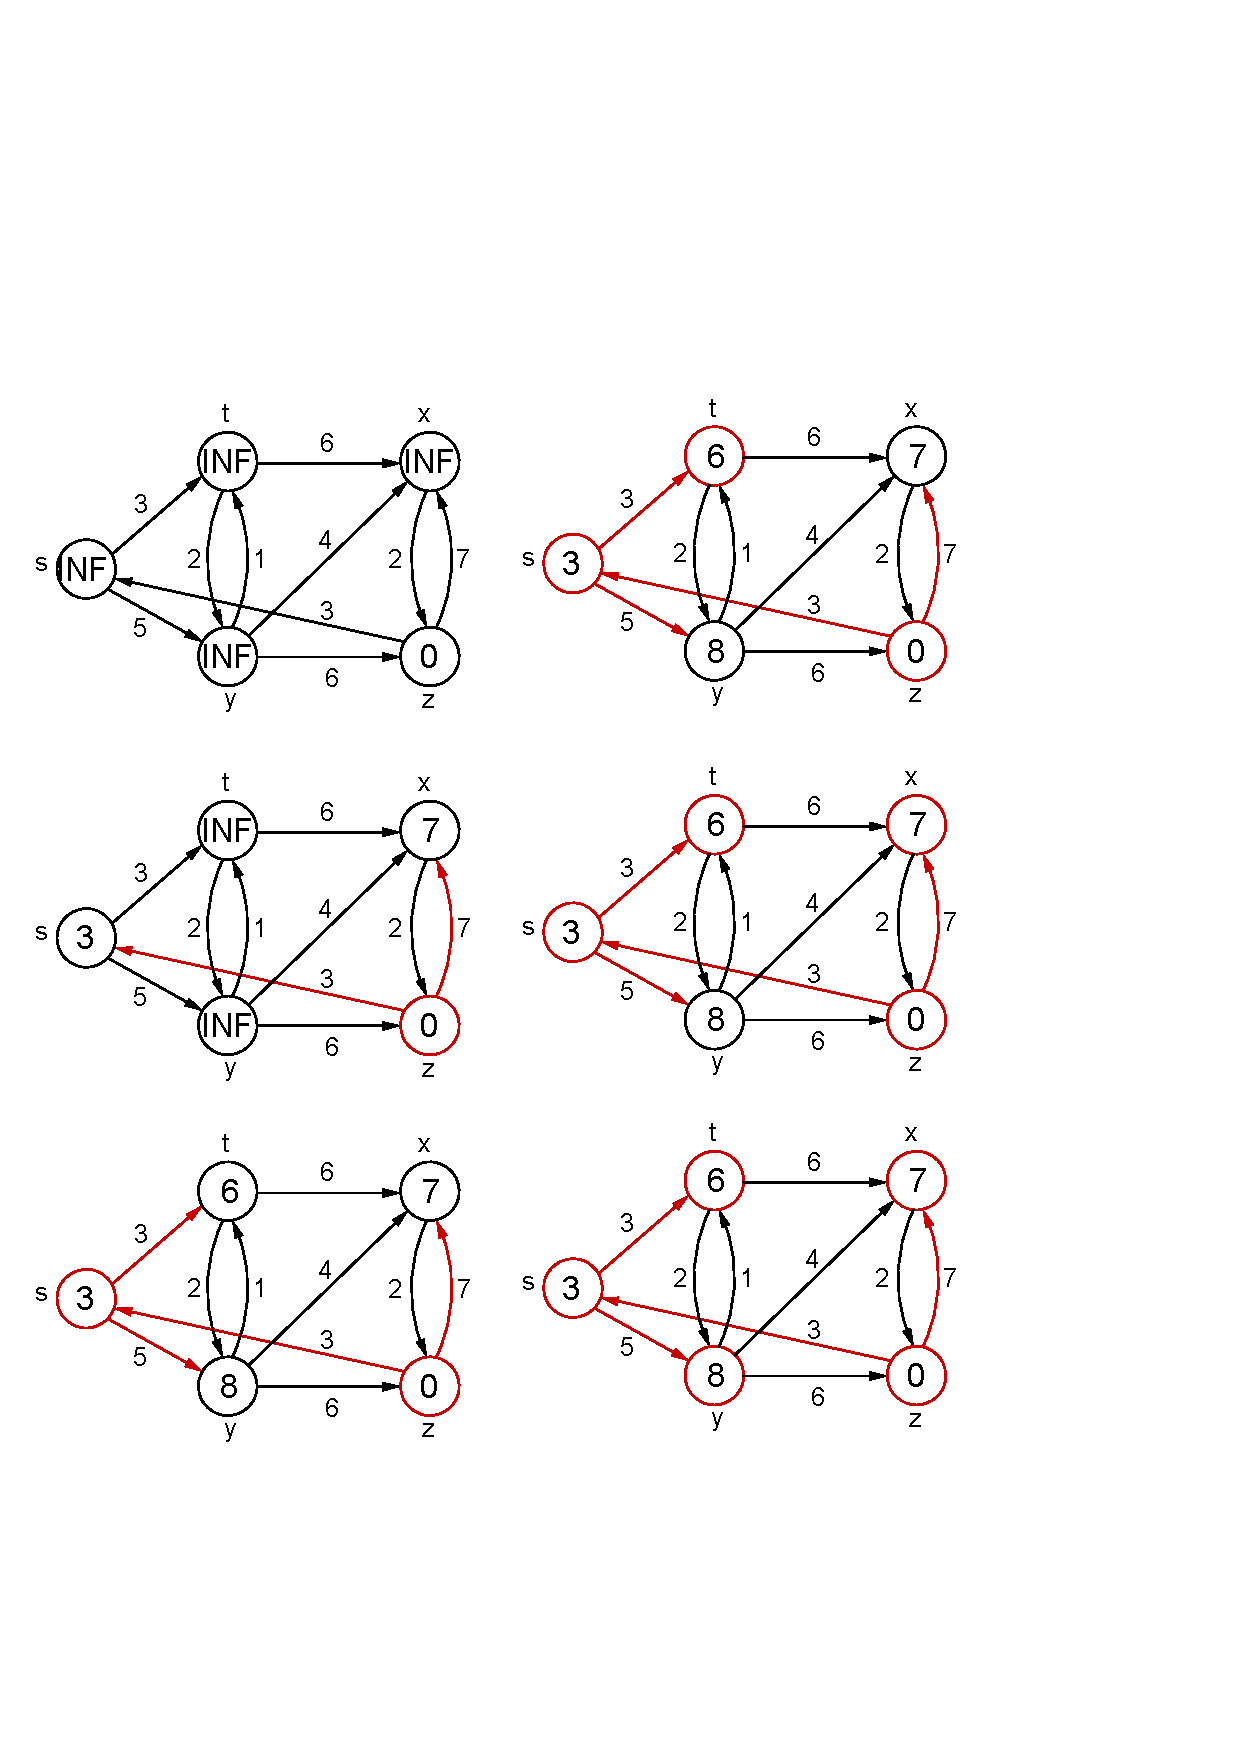
\includegraphics[width=\linewidth]{2431}
	\caption{Exercise 24.3-1}
	\label{fig:2431}
\end{figure}

\section{Question 4: CLRS Exercise 24.3-6}

Consider the modification of Dijkstra’s algorithm, growing the reliable tree from one root:

\begin{codebox}
	\Procname{$\proc{Initialize($G, root$)}$}
	\li \For each $v \in G.V$
	\li \Do	$v.d = 0$
	\li 	$v.\pi = nullptr$ \End
	\li  $root.d = 1$
\end{codebox}

\begin{codebox}
	\Procname{$\proc{Relax($u, v, r$)}$}
	\li \If $u.d < v.d * r(u, v)$ 
	\li 	\Then $u.d \leftarrow v.d * r(u, v)$
	\li  		  $v.\pi \leftarrow u$ \End
\end{codebox}

\begin{codebox}
	\Procname{$\proc{Reliable-Path-Search($G, root$)}$}
	\li \proc{Initialize($G, root$)}
	\li $Q \leftarrow G.V$	
	\li \While $!Q.empty$
	\li \Do $u = \proc{Extract-Max(Q)}$
	\li \For each $v \in G.E(u)$
	\li \Do \proc{Relax($u, v, G.r$)}
\end{codebox}

\begin{codebox}
	\Procname{$\proc{Print-Path($G, root, v$)}$}
	\li \If $v = root$
	\li \Then \Return
	\li \Else
	\li \If $v.\pi = nullptr$
	\li \Then \proc{Print(no such path)} 
	\li \Else
	\li \proc{Print-Path($G, r, v.\pi$)}
	\li \proc{Print(v)}
\end{codebox}


\section{Question 5: CLRS Exercise 25.2-1}
$
D_{0} = 
\begin{pmatrix}
	0      &\infty &\infty &\infty &-1     &\infty \\
	1      &0      &\infty &2      &\infty &\infty \\
	\infty &2      &0      &\infty &\infty &-8     \\
	-4     &\infty &\infty &0      &3      &\infty \\ 
	\infty &7      &\infty &\infty &0      &\infty \\ 
	\infty &5      &10     &\infty &\infty &0     
\end{pmatrix} \quad
D_{1} = 
\begin{pmatrix}
	0      &\infty &\infty &\infty &-1     &\infty \\
	1      &0      &\infty &2      &0      &\infty \\
	\infty &2      &0      &\infty &\infty &-8     \\
	-4     &\infty &\infty &0      &-5     &\infty \\ 
	\infty &7      &\infty &\infty &0      &\infty \\ 
	\infty &5      &10     &\infty &\infty &0     
\end{pmatrix}\\
D_{2} = 
\begin{pmatrix}
0      &\infty &\infty &\infty &-1     &\infty \\
1      &0      &\infty &2      &0      &\infty \\
3      &2      &0      &4      &2      &-8     \\
-4     &\infty &\infty &0      &-5     &\infty \\ 
8      &7      &\infty &9      &0      &\infty \\ 
6      &5      &10     &7      &5      &0     
\end{pmatrix} \quad
D_{3} = 
\begin{pmatrix}
0      &\infty &\infty &\infty &-1     &\infty \\
1      &0      &\infty &2      &0      &\infty \\
3      &2      &0      &4      &2      &-8     \\
-4     &\infty &\infty &0      &-5     &\infty \\ 
8      &7      &\infty &9      &0      &\infty \\ 
6      &5      &10     &7      &5      &0        
\end{pmatrix}	\\
D_{4} = 
\begin{pmatrix}
0      &\infty &\infty &\infty &-1     &\infty \\
-2     &0      &\infty &2      &0      &\infty \\
0      &2      &0      &4      &2      &-8     \\
-4     &\infty &\infty &0      &-5     &\infty \\ 
8      &7      &\infty &9      &0      &\infty \\ 
6      &5      &10     &7      &5      &0        
\end{pmatrix}	\quad
D_{5} = 
\begin{pmatrix}
0      &6      &\infty &8      &-1     &\infty \\
-2     &0      &\infty &2      &0      &\infty \\
0      &2      &0      &4      &2      &-8     \\
-4     &10     &\infty &0      &-5     &\infty \\ 
8      &7      &\infty &9      &0      &\infty \\ 
6      &5      &10     &7      &5      &0        
\end{pmatrix}	\\
D_{6} = 
\begin{pmatrix}
0      &6      &\infty &8      &-1     &\infty \\
-2     &0      &\infty &2      &0      &\infty \\
-2     &-3     &0      &-1     &-3     &-8     \\
-4     &10     &\infty &0      &-5     &\infty \\ 
8      &7      &\infty &9      &0      &\infty \\ 
6      &5      &10     &7      &5      &0        
\end{pmatrix}	
$
\section{Question 6: CLRS Exercise 25.2-2}
Consider the following dynamic programming function:\\
$
t_{ij}^{m} = 
\begin{cases}
	i = j & m = 0\\
	\underset{1 \le k \le n}\bigcup (t_{ik}^{m-1} \cap (w_{kj} \neq \infty)) & 1 \le m \le n-1
\end{cases}
$

\begin{codebox}
	\Procname{$\proc{Transitive-Closure-Brutal-Force($G$)}$}
	\li $n = G.V$
	\li $l[n][n][n] \leftarrow 0$
	\li \For each entry in $l[0]$
	\li \Do $l[0][i][j] \leftarrow i = j$ \End
	\li \For $m \leftarrow 1$ \To $n-1$
	\li \Do \For $i \leftarrow 1$ \To $n$
	\li \Do \For $j \leftarrow 1$ \To $n$
	\li \Do $l[m][i][j] = \underset{1 \le k \le n}\bigcup (l[m-1][i][k] \cap (G.w_{kj} \neq \infty))$
 	\End \End \End
\end{codebox}

\end{document}
